\chapter{Introduzione}
\textbf{\textit{Task}}: è un insieme di sequenze di istruzioni, che in assenza di altre attività, vengono continuamente eseguite dal processore finché non vengono completate. \\
Può essere un processo o un thread in base al sistema operativo.
\begin{center}
    \begin{tikzpicture}
        \node (1) at (-2,1)   [draw, ellipse]   {READY};
        \node (2) at (1,3)    [draw, rectangle]    {BLOCKED};
        \node (3) at (4,1)    [draw, ellipse]   {RUNNING};
        \node (4) at (-5,1)   [draw, rectangle] {activation};
        \node (5) at (7.5,1)    [draw, rectangle] {termination};
        \draw[->] (1)to[out=20,in=165,looseness=1](3)node[above]{dispacthing};
        \draw[<-] (1)to[out=340,in=200,looseness=1](3)node[below]{preemption};
        \draw[->] (3)to[out=100,in=0,looseness=1](2)node[above right]{wait};
        \draw[<-] (1)to[out=100,in=180,looseness=1](2)node[above left]{signal};
        \draw[->] (4)to(1);
        \draw[->] (3)to(5);
    \end{tikzpicture}
\end{center}

\textbf{\textit{Ready Queue}}: i task ``pronti'' (\textit{ready}) sono contenuti all'interno di una coda di attesa, anche nota come \textit{ready queue}. Le strategie con cui vengono scelti i task dalla coda per essere eseguiti sulla \textit{CPU} sono gli \textbf{\textit{scheduling algorithms}}.

\begin{center}
    \begin{tikzpicture}[node distance=3cm, every node/.style={transform shape, font=\sffamily}]
        \node (activation) [rectangle, draw, minimum width=2cm, minimum height=1cm] {activation};
        \node (queue) [rectangle, draw=none, right=of activation, minimum height=0cm] {};
        \node (cpu) [circle, draw, right=of queue, minimum size=1.5cm, inner sep=0] {CPU};
        \node (termination) [rectangle, draw, right=of cpu, minimum width=2cm, minimum height=1cm] {termination};
        
        \node[below=0.1cm of queue] (queueLabel) {\textbf{\textcolor{blue}{Ready queue}}};

        \node[block, fill=orange!20, left=0mm of queue.east, anchor=east] (tau1) {$\tau_1$};
        \node[block, fill=green!20, left=0mm of tau1, anchor=east] (tau2) {$\tau_2$};
        \node[block, fill=blue!20, left=0mm of tau2, anchor=east] (tau3) {$\tau_3$};

        \draw[->] (activation) -- (tau3);
        \draw[->] (tau1) -- node[anchor=south] {dispatching} (cpu);
        \draw[->] (cpu) -- (termination);
    \end{tikzpicture}
\end{center}
\textbf{\textit{Scheduling}} può essere definito \textbf{\textit{preemptive}} ovvero se il task in esecuzione in un certo istante di tempo $t_i$ può essere temporaneamente sospeso per eseguire un task con importanza maggiore, mentre si dice \textbf{\textit{non-preemptive}} se il task in esecuzione non può essere sospeso finché non viene completato. \\ \newline
\textbf{\textit{Schedule}}: uno \textit{schedule} è un particolare assegnamento di task ad un processore. Dato un \textbf{\textit{taskset}} $\mathcal{T} = \{\tau_1, ..., \tau_n\}$ uno \textit{schedule} viene mappato to $\sigma$: 
\begin{center}
    $\mathbb{R}^{+} \rightarrow \mathbb{N} \; | \; \forall t \in \mathbb{R}^{+} \quad $
    \begin{math}
        \sigma(t) = 
        \begin{cases}
            k>0 \quad \text{if} \; \tau_k \text{ is running} \\
            0 \qquad \;\;\; \text{if the processor is idle}
        \end{cases}
    \end{math}
\end{center}
Consideriamo il \textit{task set}: $\{\tau_1, \tau_2, \tau_3\}$
\begin{figure}[h]
    \centering
    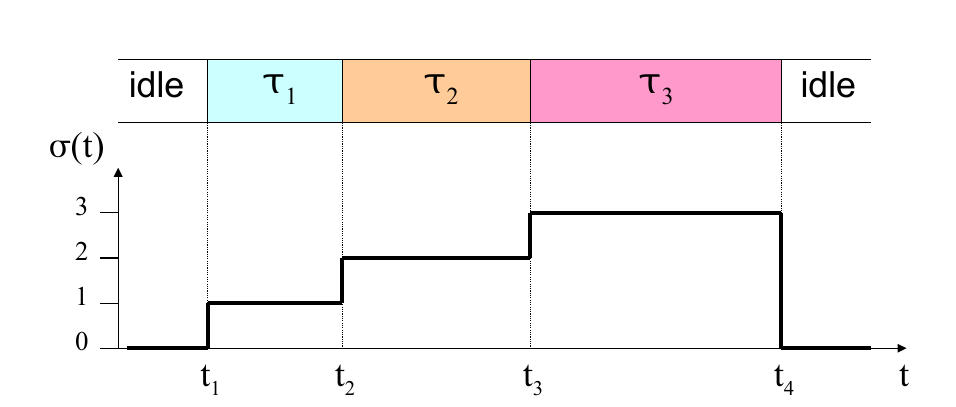
\includegraphics[width=0.5\textwidth]{img/time_sched}
\end{figure}
\newline
Nei punti $t_1$, $t_2$, $t_3$ e $t_4$ viene eseguito un \textbf{\textit{content switch}}, ogni intervallo di tempo $[t_i, t_{i+1})$ viene chiamato \textbf{\textit{time slice}}.
\begin{figure}[h]
    \centering
    \begin{minipage}[t]{0.45\textwidth}
        \centering
        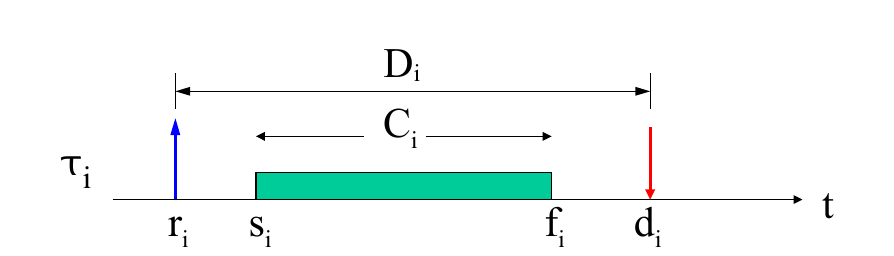
\includegraphics[width=\textwidth]{img/rt_task}
        \caption{Real-time tasks}
    \end{minipage}
    \begin{minipage}[t]{0.45\textwidth}
        \centering
        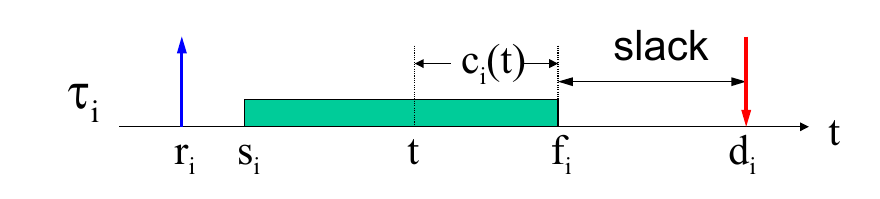
\includegraphics[width=\textwidth]{img/rt_task_1}
        \caption{Real-time tasks}
    \end{minipage}
\end{figure}
\begin{itemize}
    \item $\mathbf{r}_i$ è il \textbf{\textit{request time}}.
    \item $\mathbf{s}_i$ è lo \textbf{\textit{start time}} ovvero il tempo in cui il task inizia l'esecuzione.
    \item $\mathbf{C}_i$ è il tempo di esecuzione in caso peggiore (\textbf{\textit{WCET}}).
    \item $\mathbf{d}_i$ è la \textbf{\textit{deadline} assoluta}, mentre $\mathbf{D}_i$ è la \textbf{\textit{deadline} relativa}.
    \item $\mathbf{f}_i$ è il \textbf{\textit{finishing time}} ovvero il tempo effettivo in cui il task completa il suo lavoro
    \item \textbf{\textit{lateness}}: $L_i = f_i - d_i$, è quindi la differenza tra il tempo di fine del task e la sua deadline assoluta, se $\leq 0$ allora il task ha rispettato la sua deadline se no la deadline è stata missata [\textbf{\textit{tardiness}}: $max(0, L_i)$]
    \item \textbf{\textit{Residual WCET}}: $c_i(t)$ 
    \item \textbf{\textit{laxity (o slack)}}: $d_i - t - c_i(t)$
\end{itemize}
\textbf{\textit{Tasks vs. Jobs}}: un task è un infinita sequenza di istanze che vengono ripetute [\textit{jobs}]. È possibile differenziare varie tipologie di \textit{task} in base a quale deve essere la loro garanzia di rispetto delle loro \textit{deadline}:
\begin{enumerate}
    \item \textbf{\textit{Hard Task}}: tutti i \textit{jobs} devono rispettare le proprie deadline, mancare una deadline comporta serie conseguenze.
    \item \textbf{\textit{Firm Task}}: solo alcuni \textit{jobs} possono missare la loro deadline.
    \item \textbf{\textit{Soft Task}}: i \textit{jobs} possono missare la loro deadline, l'obiettivo è quello di massimizzare la \textbf{\textit{responsiveness}}.
\end{enumerate}
Un sistema operativo capace di gestire \textit{hard task} viene chiamato \textbf{\textit{hard real-time system}}. I \textit{tasks} possono avere due modalità di \textbf{attivazione}:
\begin{enumerate}
    \item \textbf{\textit{time driven}}: anche noti come \textbf{tasks periodici}, i task vengono automaticamente attivati dal \textit{kernel} ad intervalli regolari. Definiamo il task come: $\tau_i(C_i, T_i, D_i)$ dove $\mathbf{T_i}$ è il periodo a cui quel task viene invocato.
    \begin{center}
        \begin{math}
            \begin{cases}
                r_{i,k} = \Phi_i + (k-1) \cdot T_i \qquad k = 1 \rightarrow r_{i1}= \Phi_i \\
                d_{i,k} = r_{i,k} + D_i
            \end{cases}
        \end{math}
    \end{center}

    \item \textbf{\textit{event driven}}: anche noti come \textbf{tasks aperiodici}, ovvero il task viene attivato all'arrivo di un evento o per un'invocazione esplicita della sua primitiva di invocazione. A loro volta possono dividersi in:
    \begin{itemize}
        \item \textbf{\textit{aperiodic}}: $r_{i, k+1} > r_{i, k}$
        \item \textbf{\textit{sporadic}}: $r_{i, k+1} \geq r_{i, k} + T_i$
    \end{itemize}
\end{enumerate}
Sui \textit{tasks} possono essere imposti dei vincoli, che si differenziano in:
\begin{itemize}
    \item \textbf{\textit{timinig constraints}}: ovvero dei vincoli sul tempo di esecuzione [\textit{deadline}, \textit{activation}, \textit{completition} e \textit{jitter}], possono essere \textbf{impliciti} o \textbf{espliciti}:
    \begin{itemize}
        \item \textbf{\textit{explicit constraints}}: sono definite nelle specifiche del sistema di attivazione: apertura della valvola ogni 10s
        \item \textbf{\textit{implicit constraints}}: non appaiono nelle specifiche direttamente, ma devono essere rispettate per seguire i vincoli di utilizzo del sistema: schivare ostacoli mentre si corre ad una velocità $v$.
    \end{itemize}
    \item \textbf{\textit{precedence constraints}}: alcuni task devono rispettare delle precedenze di esecuzione, normalmente specificate da un \textbf{\textit{Directed Acyclic Graph}}:
    \begin{figure}[h]
        \centering
        \begin{minipage}[t]{0.45\textwidth}
            \centering
            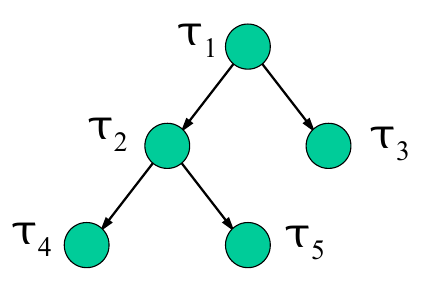
\includegraphics[width=\textwidth]{img/dag}
        \end{minipage}
        \begin{minipage}[t]{0.45\textwidth}
            \begin{center}
                predecessore \\
                $\tau_1 \prec \tau_4$ \\
                predecessore immediato \\
                $\tau_1 \rightarrow \tau_2$ \\
            \end{center}
        \end{minipage}
    \end{figure}
    \item \textbf{\textit{resource constraints}}: per preservare \textit{data consistency} bisogna accedere alle risorse condivise in \textbf{mutua esclusione}, che però introduce un \textit{delay}.
    \begin{figure}[h]
        \centering
        \begin{minipage}[t]{0.45\textwidth}
            \centering
            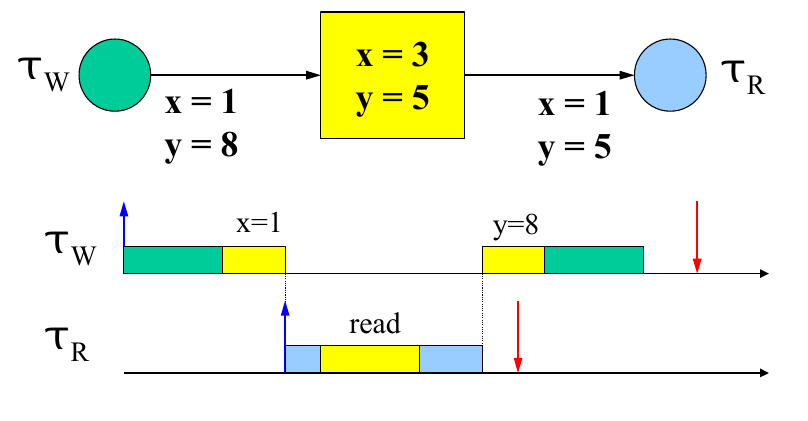
\includegraphics[width=\textwidth]{img/conc_no_me}
            \caption{\textit{no mutual exclusion}}
        \end{minipage}
        \begin{minipage}[t]{0.45\textwidth}
            \centering
            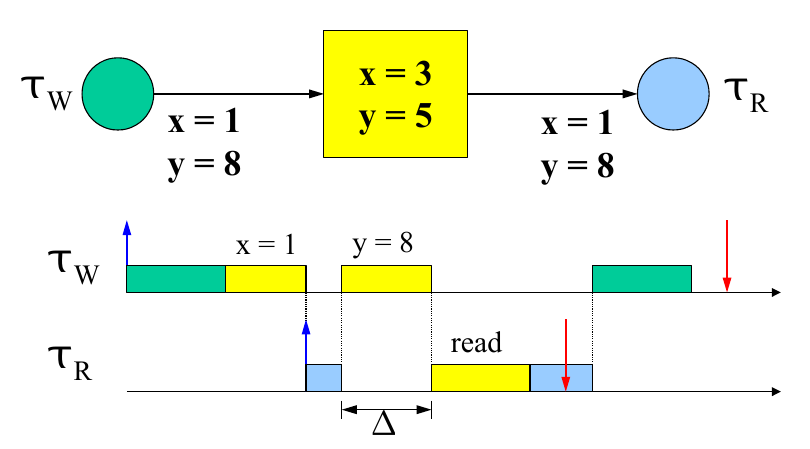
\includegraphics[width=\textwidth]{img/conc_con_me}
            \caption{\textit{mutual exclusion}}
        \end{minipage}
    \end{figure}
\end{itemize}
Mentre si analizza un \textit{tasks set} e si cerca che il tempo di esecuzion sia vincolato da vincoli imposti in fase di progettazione, ad esempio $t_r \leq 10$, anche se si aumenta il numero di processori, si diminuisce il tempo di esecuzione dei task o si rilassano i vincoli di precedenza, se non si ha uno \textbf{\textit{scheduler}} appropriato si rischia in ogni caso di missare i vincoli imposti. L'apporccio più \textbf{\textit{safe}} è quello di utilizzare meccanismi predicibili del kernel e analizzare il sistema per predirne il comportamento. La concorrenza deve essere progettata utilizzando:
\begin{itemize}
    \item appropriati algoritmi di \textbf{\textit{scheduler}}.
    \item appropriati protocolli di \textbf{sincronizzazione}.
    \item efficienti meccanismi di \textbf{comunicazione}.
    \item predicibilità negli \textbf{\textit{interrupt handling}}.
\end{itemize}
